\documentclass[11pt,fleqn]{article}
\linespread{1.3}
\usepackage{parskip}
\setlength{\parindent}{0pt} %no paragraph indentation
\setlength{\parskip}{2.1ex plus 0.2ex minus 0.2ex} %3x paragraph spacing
\usepackage{geometry}
\geometry{a4paper,left=30mm,right=25mm,top=20mm,bottom=20mm} %margin spacing
\usepackage{fancyhdr}
\pagestyle{fancy}
\fancyhf{}
\renewcommand{\headrulewidth}{0pt}
\rfoot{\thepage}

\usepackage[pdftex]{graphicx} %so that eps files may be included
\newcommand{\indep}{\rotatebox[origin=c]{90}{$\models$}} % so that \indep works :)
\usepackage[fleqn]{amsmath}
\usepackage{amssymb}
\usepackage{amsthm}
\usepackage{float}
\usepackage[bottom]{footmisc}

% Theorems, definitions etc.
\newtheoremstyle{defstyle}
  {10pt} % Space above
  {0pt} % Space below
  {} % Body font
  {} % Indent amount
  {\bfseries} % Theorem head font
  {.} % Punctuation after theorem head
  {0.5em} % Space after theorem head
  {} % Theorem head spec (can be left empty, meaning `normal')
\theoremstyle{defstyle}
\newtheorem{defn}{Definition}[section]
\newtheorem{rmrk}{Remark}[section]
\newtheorem{thrm}{Theorem}[section]
\newtheorem{ax}{Axiom}[section]

\usepackage{comment}

\usepackage{tikz}
\usetikzlibrary{bayesnet}
\begin{document}

\section{Hidden Markov Models}
\label{sec_hmm}
In this section we consider probabilistic Graphical Models of the form shown in Figure \ref{fig_linmod}. We assume that  $X_0, X_1,...$ are each $n$ state discrete random variables and that $Y_0, Y_1,...$ are each $m$ state discrete random variables. Models of this form are classically called Hidden Markov Models (HMMs).
\begin{figure}[H] 
\centering
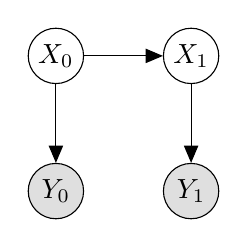
\begin{tikzpicture}

  % Define nodes
  \node[obs] (ya) {$Y_{0}$};
  \node[latent, above=of ya]  (xa) {$X_{0}$};
  \node[obs, right=of ya] (yb) {$Y_{1}$};
  \node[latent, above=of yb, right=of xa]  (xb) {$X_1$};
  
  % Connect the nodes
  \edge {xa} {ya};
  \edge {xa} {xb};
  \edge {xb} {yb};
  
\end{tikzpicture}
\caption{Graphical model of this section}
\label{fig_linmod}
\end{figure}
Intuitively, this model represents the situation where we are not sure 
\end{document}